\documentclass[twoside]{book}

% Packages required by doxygen
\usepackage{fixltx2e}
\usepackage{calc}
\usepackage{doxygen}
\usepackage[export]{adjustbox} % also loads graphicx
\usepackage{graphicx}
\usepackage[utf8]{inputenc}
\usepackage{makeidx}
\usepackage{multicol}
\usepackage{multirow}
\PassOptionsToPackage{warn}{textcomp}
\usepackage{textcomp}
\usepackage[nointegrals]{wasysym}
\usepackage[table]{xcolor}

% Font selection
\usepackage[T1]{fontenc}
\usepackage[scaled=.90]{helvet}
\usepackage{courier}
\usepackage{amssymb}
\usepackage{sectsty}
\renewcommand{\familydefault}{\sfdefault}
\allsectionsfont{%
  \fontseries{bc}\selectfont%
  \color{darkgray}%
}
\renewcommand{\DoxyLabelFont}{%
  \fontseries{bc}\selectfont%
  \color{darkgray}%
}
\newcommand{\+}{\discretionary{\mbox{\scriptsize$\hookleftarrow$}}{}{}}

% Page & text layout
\usepackage{geometry}
\geometry{%
  a4paper,%
  top=2.5cm,%
  bottom=2.5cm,%
  left=2.5cm,%
  right=2.5cm%
}
\tolerance=750
\hfuzz=15pt
\hbadness=750
\setlength{\emergencystretch}{15pt}
\setlength{\parindent}{0cm}
\setlength{\parskip}{3ex plus 2ex minus 2ex}
\makeatletter
\renewcommand{\paragraph}{%
  \@startsection{paragraph}{4}{0ex}{-1.0ex}{1.0ex}{%
    \normalfont\normalsize\bfseries\SS@parafont%
  }%
}
\renewcommand{\subparagraph}{%
  \@startsection{subparagraph}{5}{0ex}{-1.0ex}{1.0ex}{%
    \normalfont\normalsize\bfseries\SS@subparafont%
  }%
}
\makeatother

% Headers & footers
\usepackage{fancyhdr}
\pagestyle{fancyplain}
\fancyhead[LE]{\fancyplain{}{\bfseries\thepage}}
\fancyhead[CE]{\fancyplain{}{}}
\fancyhead[RE]{\fancyplain{}{\bfseries\leftmark}}
\fancyhead[LO]{\fancyplain{}{\bfseries\rightmark}}
\fancyhead[CO]{\fancyplain{}{}}
\fancyhead[RO]{\fancyplain{}{\bfseries\thepage}}
\fancyfoot[LE]{\fancyplain{}{}}
\fancyfoot[CE]{\fancyplain{}{}}
\fancyfoot[RE]{\fancyplain{}{\bfseries\scriptsize Generated by Doxygen }}
\fancyfoot[LO]{\fancyplain{}{\bfseries\scriptsize Generated by Doxygen }}
\fancyfoot[CO]{\fancyplain{}{}}
\fancyfoot[RO]{\fancyplain{}{}}
\renewcommand{\footrulewidth}{0.4pt}
\renewcommand{\chaptermark}[1]{%
  \markboth{#1}{}%
}
\renewcommand{\sectionmark}[1]{%
  \markright{\thesection\ #1}%
}

% Indices & bibliography
\usepackage{natbib}
\usepackage[titles]{tocloft}
\setcounter{tocdepth}{3}
\setcounter{secnumdepth}{5}
\makeindex

% Hyperlinks (required, but should be loaded last)
\usepackage{ifpdf}
\ifpdf
  \usepackage[pdftex,pagebackref=true]{hyperref}
\else
  \usepackage[ps2pdf,pagebackref=true]{hyperref}
\fi
\hypersetup{%
  colorlinks=true,%
  linkcolor=blue,%
  citecolor=blue,%
  unicode%
}

% Custom commands
\newcommand{\clearemptydoublepage}{%
  \newpage{\pagestyle{empty}\cleardoublepage}%
}

\usepackage{caption}
\captionsetup{labelsep=space,justification=centering,font={bf},singlelinecheck=off,skip=4pt,position=top}

%===== C O N T E N T S =====

\begin{document}

% Titlepage & ToC
\hypersetup{pageanchor=false,
             bookmarksnumbered=true,
             pdfencoding=unicode
            }
\pagenumbering{alph}
\begin{titlepage}
\vspace*{7cm}
\begin{center}%
{\Large Project 2 }\\
\vspace*{1cm}
{\large Generated by Doxygen 1.8.13}\\
\end{center}
\end{titlepage}
\clearemptydoublepage
\pagenumbering{roman}
\tableofcontents
\clearemptydoublepage
\pagenumbering{arabic}
\hypersetup{pageanchor=true}

%--- Begin generated contents ---
\chapter{Hierarchical Index}
\section{Class Hierarchy}
This inheritance list is sorted roughly, but not completely, alphabetically\+:\begin{DoxyCompactList}
\item \contentsline{section}{Base\+Map}{\pageref{class_base_map}}{}
\begin{DoxyCompactList}
\item \contentsline{section}{Map1}{\pageref{class_map1}}{}
\item \contentsline{section}{Map2}{\pageref{class_map2}}{}
\item \contentsline{section}{Map3}{\pageref{class_map3}}{}
\end{DoxyCompactList}
\item \contentsline{section}{Object}{\pageref{class_object}}{}
\begin{DoxyCompactList}
\item \contentsline{section}{Fruit}{\pageref{class_fruit}}{}
\item \contentsline{section}{List\+Node}{\pageref{class_list_node}}{}
\item \contentsline{section}{Walls}{\pageref{class_walls}}{}
\end{DoxyCompactList}
\item \contentsline{section}{Scores}{\pageref{struct_scores}}{}
\item \contentsline{section}{Snake}{\pageref{class_snake}}{}
\end{DoxyCompactList}

\chapter{Class Index}
\section{Class List}
Here are the classes, structs, unions and interfaces with brief descriptions\+:\begin{DoxyCompactList}
\item\contentsline{section}{\hyperlink{struct_scores}{Scores} }{\pageref{struct_scores}}{}
\end{DoxyCompactList}

\chapter{Class Documentation}
\hypertarget{class_base_map}{}\section{Base\+Map Class Reference}
\label{class_base_map}\index{Base\+Map@{Base\+Map}}
Inheritance diagram for Base\+Map\+:\begin{figure}[H]
\begin{center}
\leavevmode
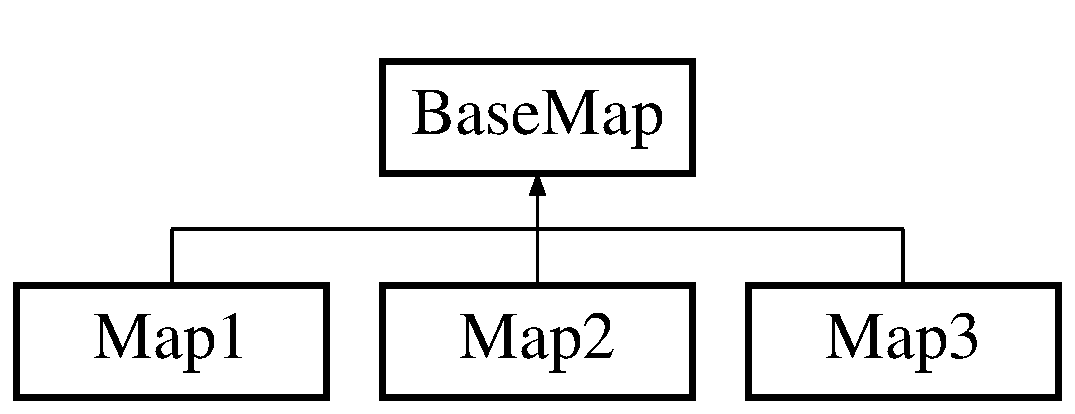
\includegraphics[height=2.000000cm]{class_base_map}
\end{center}
\end{figure}
\subsection*{Public Member Functions}
\begin{DoxyCompactItemize}
\item 
\hyperlink{class_base_map_a00dd2d0f12517f43d8c046a4d8b681bf}{Base\+Map} ()
\begin{DoxyCompactList}\small\item\em Constructor of \hyperlink{class_base_map}{Base\+Map} class. \end{DoxyCompactList}\end{DoxyCompactItemize}
\subsection*{Public Attributes}
\begin{DoxyCompactItemize}
\item 
\hyperlink{class_object}{Object} \hyperlink{class_base_map_a1d9ea4ce08a8bbd32ac24ccead7a546d}{map} \mbox{[}30\mbox{]}\mbox{[}60\mbox{]}
\end{DoxyCompactItemize}


\subsection{Constructor \& Destructor Documentation}
\mbox{\Hypertarget{class_base_map_a00dd2d0f12517f43d8c046a4d8b681bf}\label{class_base_map_a00dd2d0f12517f43d8c046a4d8b681bf}} 
\index{Base\+Map@{Base\+Map}!Base\+Map@{Base\+Map}}
\index{Base\+Map@{Base\+Map}!Base\+Map@{Base\+Map}}
\subsubsection{\texorpdfstring{Base\+Map()}{BaseMap()}}
{\footnotesize\ttfamily Base\+Map\+::\+Base\+Map (\begin{DoxyParamCaption}{ }\end{DoxyParamCaption})}



Constructor of \hyperlink{class_base_map}{Base\+Map} class. 


\begin{DoxyParams}{Parameters}
{\em none} & \\
\hline
\end{DoxyParams}
\begin{DoxyReturn}{Returns}
none 
\end{DoxyReturn}


\subsection{Member Data Documentation}
\mbox{\Hypertarget{class_base_map_a1d9ea4ce08a8bbd32ac24ccead7a546d}\label{class_base_map_a1d9ea4ce08a8bbd32ac24ccead7a546d}} 
\index{Base\+Map@{Base\+Map}!map@{map}}
\index{map@{map}!Base\+Map@{Base\+Map}}
\subsubsection{\texorpdfstring{map}{map}}
{\footnotesize\ttfamily \hyperlink{class_object}{Object} Base\+Map\+::map\mbox{[}30\mbox{]}\mbox{[}60\mbox{]}}

Node of map 

The documentation for this class was generated from the following files\+:\begin{DoxyCompactItemize}
\item 
D\+:/\+R\+C\+C/\+C\+I\+S17\+A/\+Mac\+Nhan\+\_\+44051/\+Proj/\+Project\+\_\+2/\+Project2/Base\+Map.\+h\item 
D\+:/\+R\+C\+C/\+C\+I\+S17\+A/\+Mac\+Nhan\+\_\+44051/\+Proj/\+Project\+\_\+2/\+Project2/Base\+Map.\+cpp\end{DoxyCompactItemize}

\hypertarget{class_fruit}{}\section{Fruit Class Reference}
\label{class_fruit}\index{Fruit@{Fruit}}
Inheritance diagram for Fruit\+:\begin{figure}[H]
\begin{center}
\leavevmode
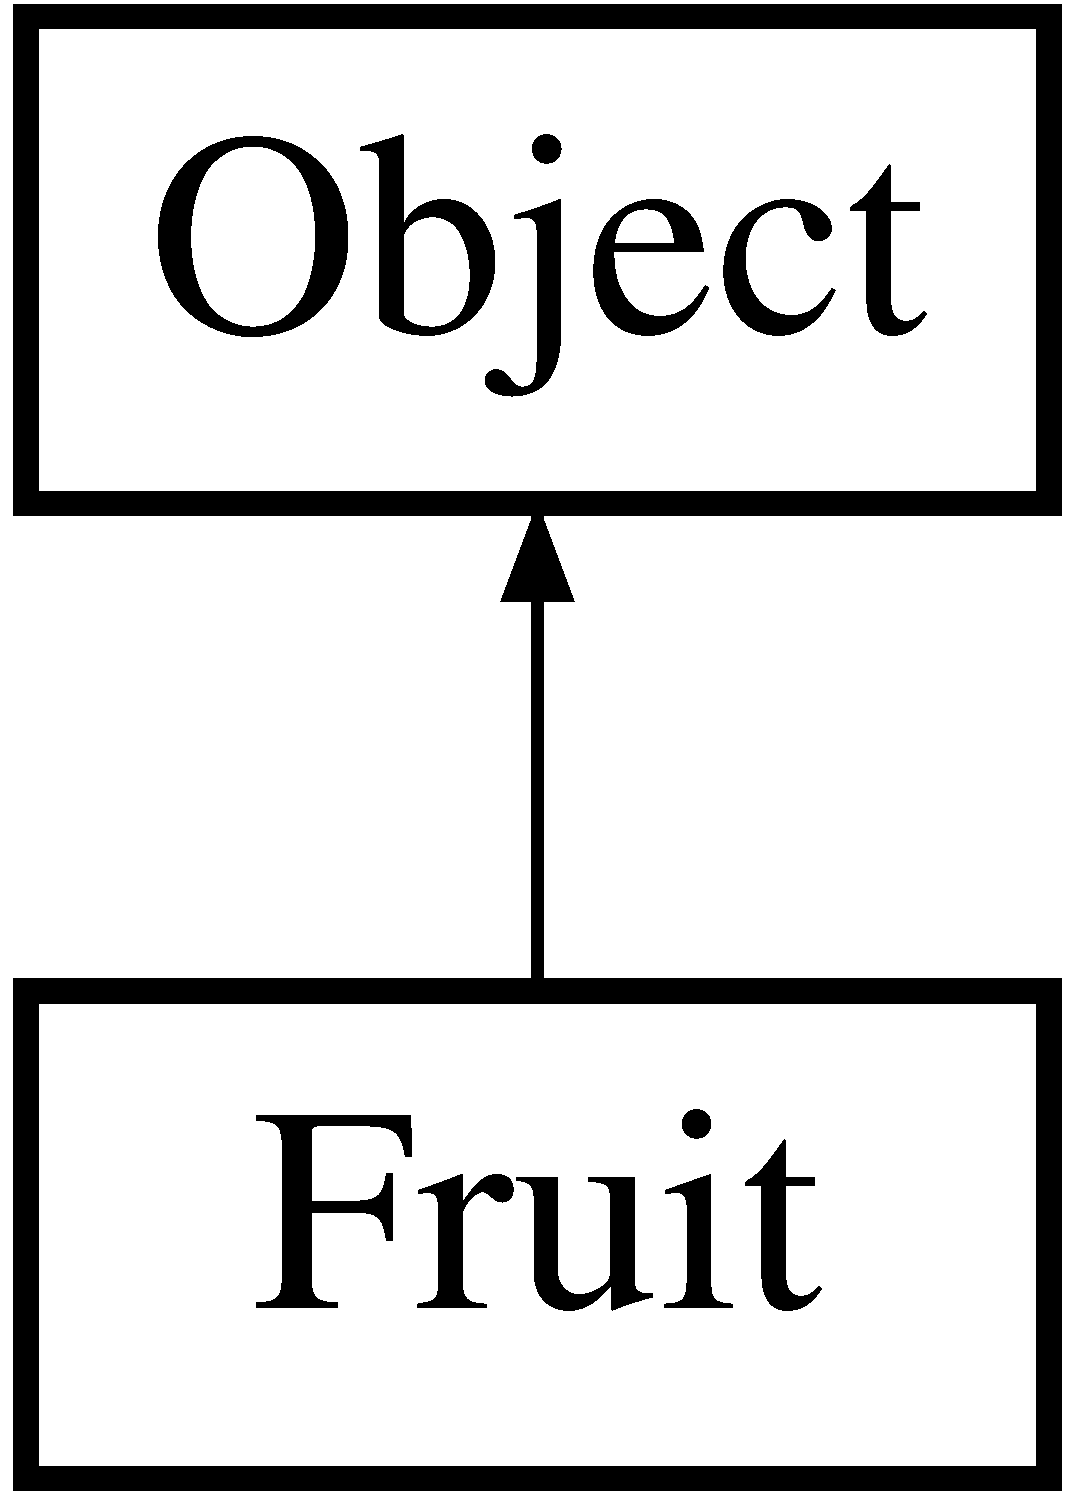
\includegraphics[height=2.000000cm]{class_fruit}
\end{center}
\end{figure}
\subsection*{Public Member Functions}
\begin{DoxyCompactItemize}
\item 
\hyperlink{class_fruit_aa40ce1fdb1b361880d27171f05a2ab5a}{Fruit} ()
\begin{DoxyCompactList}\small\item\em Constructor of \hyperlink{class_fruit}{Fruit} class. \end{DoxyCompactList}\item 
void \hyperlink{class_fruit_a1fdcbedbadc7809aceaffd4164754c25}{re\+Location} ()
\begin{DoxyCompactList}\small\item\em re\+Location function is a function generation coordinates x,y \end{DoxyCompactList}\end{DoxyCompactItemize}
\subsection*{Additional Inherited Members}


\subsection{Constructor \& Destructor Documentation}
\mbox{\Hypertarget{class_fruit_aa40ce1fdb1b361880d27171f05a2ab5a}\label{class_fruit_aa40ce1fdb1b361880d27171f05a2ab5a}} 
\index{Fruit@{Fruit}!Fruit@{Fruit}}
\index{Fruit@{Fruit}!Fruit@{Fruit}}
\subsubsection{\texorpdfstring{Fruit()}{Fruit()}}
{\footnotesize\ttfamily Fruit\+::\+Fruit (\begin{DoxyParamCaption}{ }\end{DoxyParamCaption})}



Constructor of \hyperlink{class_fruit}{Fruit} class. 


\begin{DoxyParams}{Parameters}
{\em none} & \\
\hline
\end{DoxyParams}
\begin{DoxyReturn}{Returns}
none 
\end{DoxyReturn}


\subsection{Member Function Documentation}
\mbox{\Hypertarget{class_fruit_a1fdcbedbadc7809aceaffd4164754c25}\label{class_fruit_a1fdcbedbadc7809aceaffd4164754c25}} 
\index{Fruit@{Fruit}!re\+Location@{re\+Location}}
\index{re\+Location@{re\+Location}!Fruit@{Fruit}}
\subsubsection{\texorpdfstring{re\+Location()}{reLocation()}}
{\footnotesize\ttfamily void Fruit\+::re\+Location (\begin{DoxyParamCaption}{ }\end{DoxyParamCaption})}



re\+Location function is a function generation coordinates x,y 


\begin{DoxyParams}{Parameters}
{\em none} & \\
\hline
\end{DoxyParams}
\begin{DoxyReturn}{Returns}
none 
\end{DoxyReturn}


The documentation for this class was generated from the following files\+:\begin{DoxyCompactItemize}
\item 
D\+:/\+R\+C\+C/\+C\+I\+S17\+A/\+Mac\+Nhan\+\_\+44051/\+Proj/\+Project\+\_\+2/\+Project2/Fruit.\+h\item 
D\+:/\+R\+C\+C/\+C\+I\+S17\+A/\+Mac\+Nhan\+\_\+44051/\+Proj/\+Project\+\_\+2/\+Project2/Fruit.\+cpp\end{DoxyCompactItemize}

\hypertarget{class_list_node}{}\section{List\+Node Class Reference}
\label{class_list_node}\index{List\+Node@{List\+Node}}
Inheritance diagram for List\+Node\+:\begin{figure}[H]
\begin{center}
\leavevmode
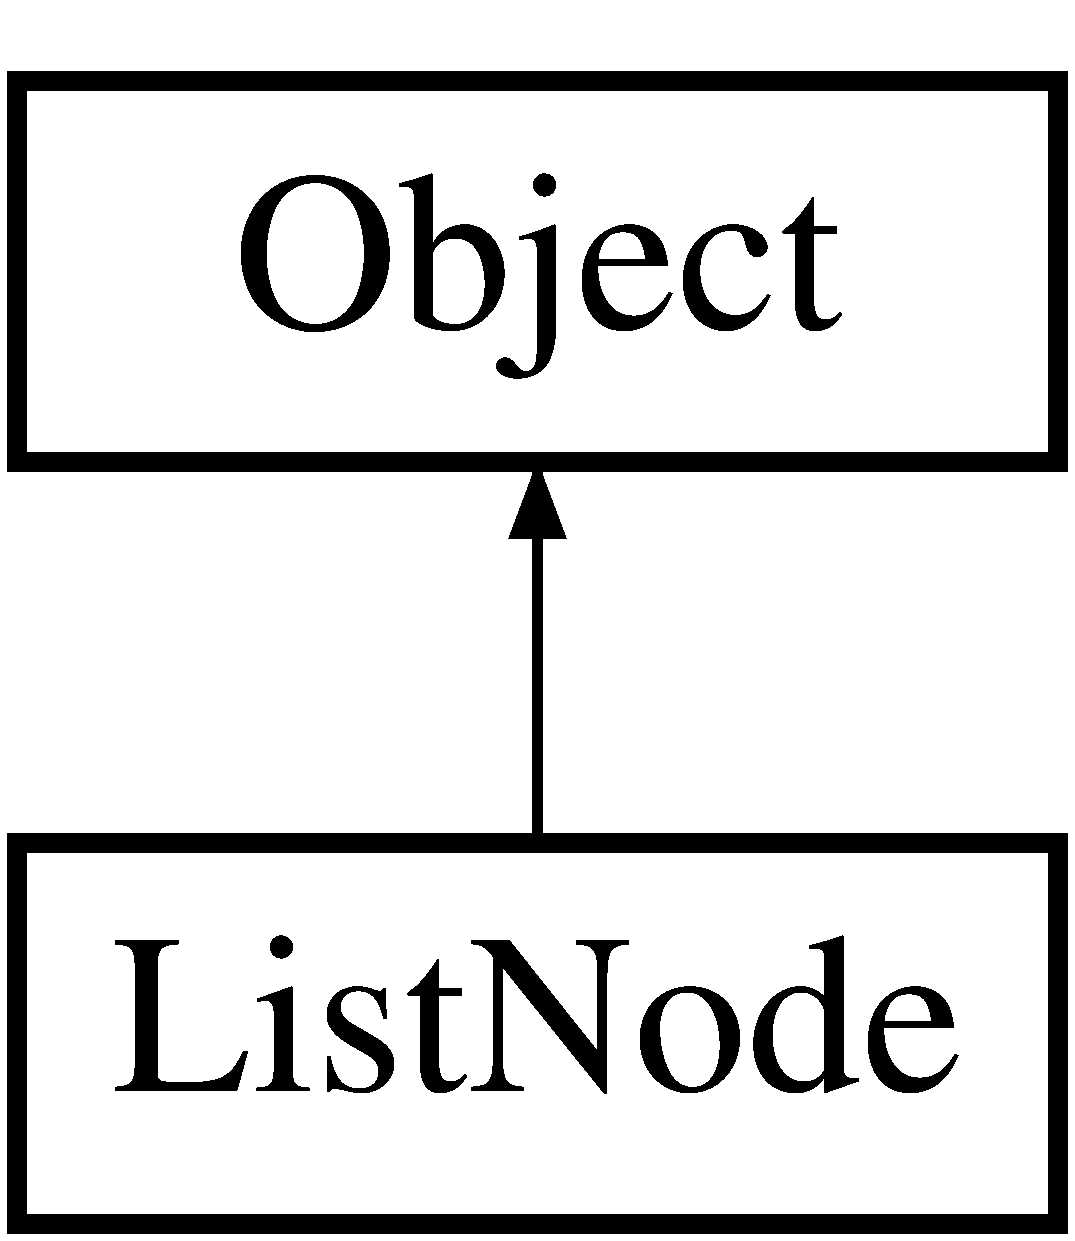
\includegraphics[height=2.000000cm]{class_list_node}
\end{center}
\end{figure}
\subsection*{Public Member Functions}
\begin{DoxyCompactItemize}
\item 
\hyperlink{class_list_node_ac8e8674ba4da13a5074bfdf49471c585}{List\+Node} ()
\begin{DoxyCompactList}\small\item\em Constructor of \hyperlink{class_list_node}{List\+Node} class. \end{DoxyCompactList}\item 
\hyperlink{class_list_node_a40fa34640e78f3d0bcb576feb52edcaf}{List\+Node} (bool)
\begin{DoxyCompactList}\small\item\em Constructor of \hyperlink{class_list_node}{List\+Node} class. \end{DoxyCompactList}\item 
\hyperlink{class_list_node}{List\+Node} $\ast$ \hyperlink{class_list_node_a67d0812638ee0cf0504c4e26300140f4}{get\+Next\+Node} ()
\begin{DoxyCompactList}\small\item\em Get the next node. \end{DoxyCompactList}\item 
\hyperlink{class_list_node}{List\+Node} $\ast$ \hyperlink{class_list_node_ac9da9956959adb42c1208090358b27a9}{get\+Previous\+Node} ()
\begin{DoxyCompactList}\small\item\em Get the previous node. \end{DoxyCompactList}\item 
void \hyperlink{class_list_node_aea1731114341126c371cd2fa5f674a11}{set\+Next\+Node} (\hyperlink{class_list_node}{List\+Node} $\ast$)
\begin{DoxyCompactList}\small\item\em set the value of next node \end{DoxyCompactList}\item 
void \hyperlink{class_list_node_aa45816b74681f1b3765003477b5f2771}{set\+Previous\+Node} (\hyperlink{class_list_node}{List\+Node} $\ast$)
\begin{DoxyCompactList}\small\item\em set the value of previous node \end{DoxyCompactList}\end{DoxyCompactItemize}
\subsection*{Additional Inherited Members}


\subsection{Constructor \& Destructor Documentation}
\mbox{\Hypertarget{class_list_node_ac8e8674ba4da13a5074bfdf49471c585}\label{class_list_node_ac8e8674ba4da13a5074bfdf49471c585}} 
\index{List\+Node@{List\+Node}!List\+Node@{List\+Node}}
\index{List\+Node@{List\+Node}!List\+Node@{List\+Node}}
\subsubsection{\texorpdfstring{List\+Node()}{ListNode()}\hspace{0.1cm}{\footnotesize\ttfamily [1/2]}}
{\footnotesize\ttfamily List\+Node\+::\+List\+Node (\begin{DoxyParamCaption}{ }\end{DoxyParamCaption})}



Constructor of \hyperlink{class_list_node}{List\+Node} class. 


\begin{DoxyParams}{Parameters}
{\em none} & \\
\hline
\end{DoxyParams}
\begin{DoxyReturn}{Returns}
none 
\end{DoxyReturn}
\mbox{\Hypertarget{class_list_node_a40fa34640e78f3d0bcb576feb52edcaf}\label{class_list_node_a40fa34640e78f3d0bcb576feb52edcaf}} 
\index{List\+Node@{List\+Node}!List\+Node@{List\+Node}}
\index{List\+Node@{List\+Node}!List\+Node@{List\+Node}}
\subsubsection{\texorpdfstring{List\+Node()}{ListNode()}\hspace{0.1cm}{\footnotesize\ttfamily [2/2]}}
{\footnotesize\ttfamily List\+Node\+::\+List\+Node (\begin{DoxyParamCaption}\item[{bool}]{is\+Head }\end{DoxyParamCaption})}



Constructor of \hyperlink{class_list_node}{List\+Node} class. 


\begin{DoxyParams}{Parameters}
{\em is\+Head} & -\/ A flag notice this node is the head \\
\hline
\end{DoxyParams}
\begin{DoxyReturn}{Returns}
none 
\end{DoxyReturn}


\subsection{Member Function Documentation}
\mbox{\Hypertarget{class_list_node_a67d0812638ee0cf0504c4e26300140f4}\label{class_list_node_a67d0812638ee0cf0504c4e26300140f4}} 
\index{List\+Node@{List\+Node}!get\+Next\+Node@{get\+Next\+Node}}
\index{get\+Next\+Node@{get\+Next\+Node}!List\+Node@{List\+Node}}
\subsubsection{\texorpdfstring{get\+Next\+Node()}{getNextNode()}}
{\footnotesize\ttfamily \hyperlink{class_list_node}{List\+Node} $\ast$ List\+Node\+::get\+Next\+Node (\begin{DoxyParamCaption}{ }\end{DoxyParamCaption})}



Get the next node. 


\begin{DoxyParams}{Parameters}
{\em none} & \\
\hline
\end{DoxyParams}
\begin{DoxyReturn}{Returns}
none 
\end{DoxyReturn}
\mbox{\Hypertarget{class_list_node_ac9da9956959adb42c1208090358b27a9}\label{class_list_node_ac9da9956959adb42c1208090358b27a9}} 
\index{List\+Node@{List\+Node}!get\+Previous\+Node@{get\+Previous\+Node}}
\index{get\+Previous\+Node@{get\+Previous\+Node}!List\+Node@{List\+Node}}
\subsubsection{\texorpdfstring{get\+Previous\+Node()}{getPreviousNode()}}
{\footnotesize\ttfamily \hyperlink{class_list_node}{List\+Node} $\ast$ List\+Node\+::get\+Previous\+Node (\begin{DoxyParamCaption}{ }\end{DoxyParamCaption})}



Get the previous node. 


\begin{DoxyParams}{Parameters}
{\em none} & \\
\hline
\end{DoxyParams}
\begin{DoxyReturn}{Returns}
none 
\end{DoxyReturn}
\mbox{\Hypertarget{class_list_node_aea1731114341126c371cd2fa5f674a11}\label{class_list_node_aea1731114341126c371cd2fa5f674a11}} 
\index{List\+Node@{List\+Node}!set\+Next\+Node@{set\+Next\+Node}}
\index{set\+Next\+Node@{set\+Next\+Node}!List\+Node@{List\+Node}}
\subsubsection{\texorpdfstring{set\+Next\+Node()}{setNextNode()}}
{\footnotesize\ttfamily void List\+Node\+::set\+Next\+Node (\begin{DoxyParamCaption}\item[{\hyperlink{class_list_node}{List\+Node} $\ast$}]{new\+Node }\end{DoxyParamCaption})}



set the value of next node 


\begin{DoxyParams}{Parameters}
{\em new\+Node} & -\/ The value of next node \\
\hline
\end{DoxyParams}
\begin{DoxyReturn}{Returns}
none 
\end{DoxyReturn}
\mbox{\Hypertarget{class_list_node_aa45816b74681f1b3765003477b5f2771}\label{class_list_node_aa45816b74681f1b3765003477b5f2771}} 
\index{List\+Node@{List\+Node}!set\+Previous\+Node@{set\+Previous\+Node}}
\index{set\+Previous\+Node@{set\+Previous\+Node}!List\+Node@{List\+Node}}
\subsubsection{\texorpdfstring{set\+Previous\+Node()}{setPreviousNode()}}
{\footnotesize\ttfamily void List\+Node\+::set\+Previous\+Node (\begin{DoxyParamCaption}\item[{\hyperlink{class_list_node}{List\+Node} $\ast$}]{new\+Node }\end{DoxyParamCaption})}



set the value of previous node 


\begin{DoxyParams}{Parameters}
{\em new\+Node} & -\/ The value of previous node \\
\hline
\end{DoxyParams}
\begin{DoxyReturn}{Returns}
none 
\end{DoxyReturn}


The documentation for this class was generated from the following files\+:\begin{DoxyCompactItemize}
\item 
D\+:/\+R\+C\+C/\+C\+I\+S17\+A/\+Mac\+Nhan\+\_\+44051/\+Proj/\+Project\+\_\+2/\+Project2/List\+Node.\+h\item 
D\+:/\+R\+C\+C/\+C\+I\+S17\+A/\+Mac\+Nhan\+\_\+44051/\+Proj/\+Project\+\_\+2/\+Project2/List\+Node.\+cpp\end{DoxyCompactItemize}

\hypertarget{class_map1}{}\section{Map1 Class Reference}
\label{class_map1}\index{Map1@{Map1}}
Inheritance diagram for Map1\+:\begin{figure}[H]
\begin{center}
\leavevmode
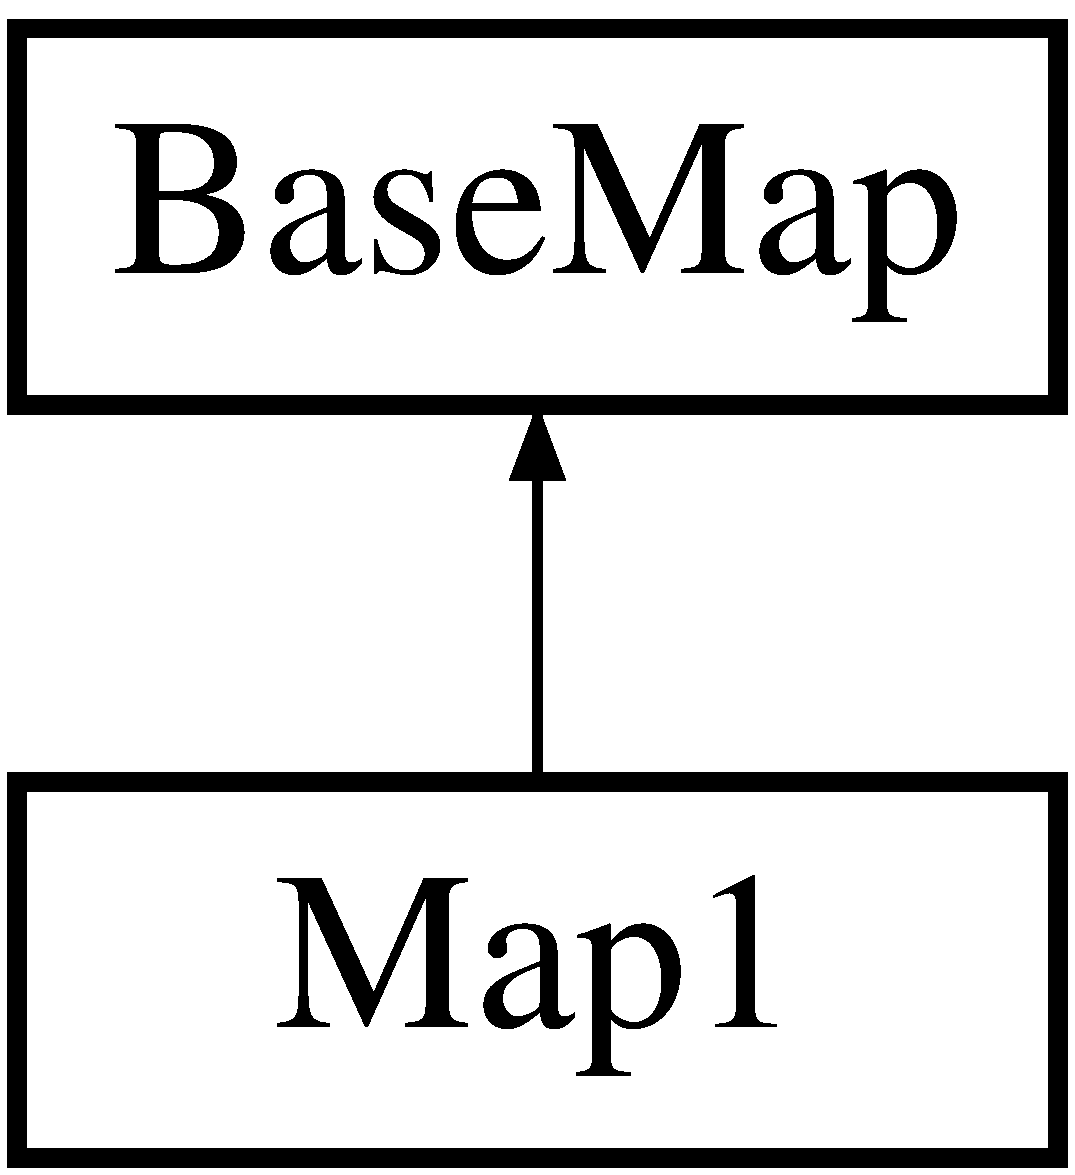
\includegraphics[height=2.000000cm]{class_map1}
\end{center}
\end{figure}
\subsection*{Public Member Functions}
\begin{DoxyCompactItemize}
\item 
\hyperlink{class_map1_a906bd64b53d0bc4cd04ce143fe2f9d2b}{Map1} ()
\begin{DoxyCompactList}\small\item\em Constructor of \hyperlink{class_map1}{Map1} class. \end{DoxyCompactList}\end{DoxyCompactItemize}
\subsection*{Additional Inherited Members}


\subsection{Constructor \& Destructor Documentation}
\mbox{\Hypertarget{class_map1_a906bd64b53d0bc4cd04ce143fe2f9d2b}\label{class_map1_a906bd64b53d0bc4cd04ce143fe2f9d2b}} 
\index{Map1@{Map1}!Map1@{Map1}}
\index{Map1@{Map1}!Map1@{Map1}}
\subsubsection{\texorpdfstring{Map1()}{Map1()}}
{\footnotesize\ttfamily Map1\+::\+Map1 (\begin{DoxyParamCaption}{ }\end{DoxyParamCaption})}



Constructor of \hyperlink{class_map1}{Map1} class. 


\begin{DoxyParams}{Parameters}
{\em none} & \\
\hline
\end{DoxyParams}
\begin{DoxyReturn}{Returns}
none 
\end{DoxyReturn}


The documentation for this class was generated from the following files\+:\begin{DoxyCompactItemize}
\item 
D\+:/\+R\+C\+C/\+C\+I\+S17\+A/\+Mac\+Nhan\+\_\+44051/\+Proj/\+Project\+\_\+2/\+Project2/Map1.\+h\item 
D\+:/\+R\+C\+C/\+C\+I\+S17\+A/\+Mac\+Nhan\+\_\+44051/\+Proj/\+Project\+\_\+2/\+Project2/Map1.\+cpp\end{DoxyCompactItemize}

\hypertarget{class_map2}{}\section{Map2 Class Reference}
\label{class_map2}\index{Map2@{Map2}}
Inheritance diagram for Map2\+:\begin{figure}[H]
\begin{center}
\leavevmode
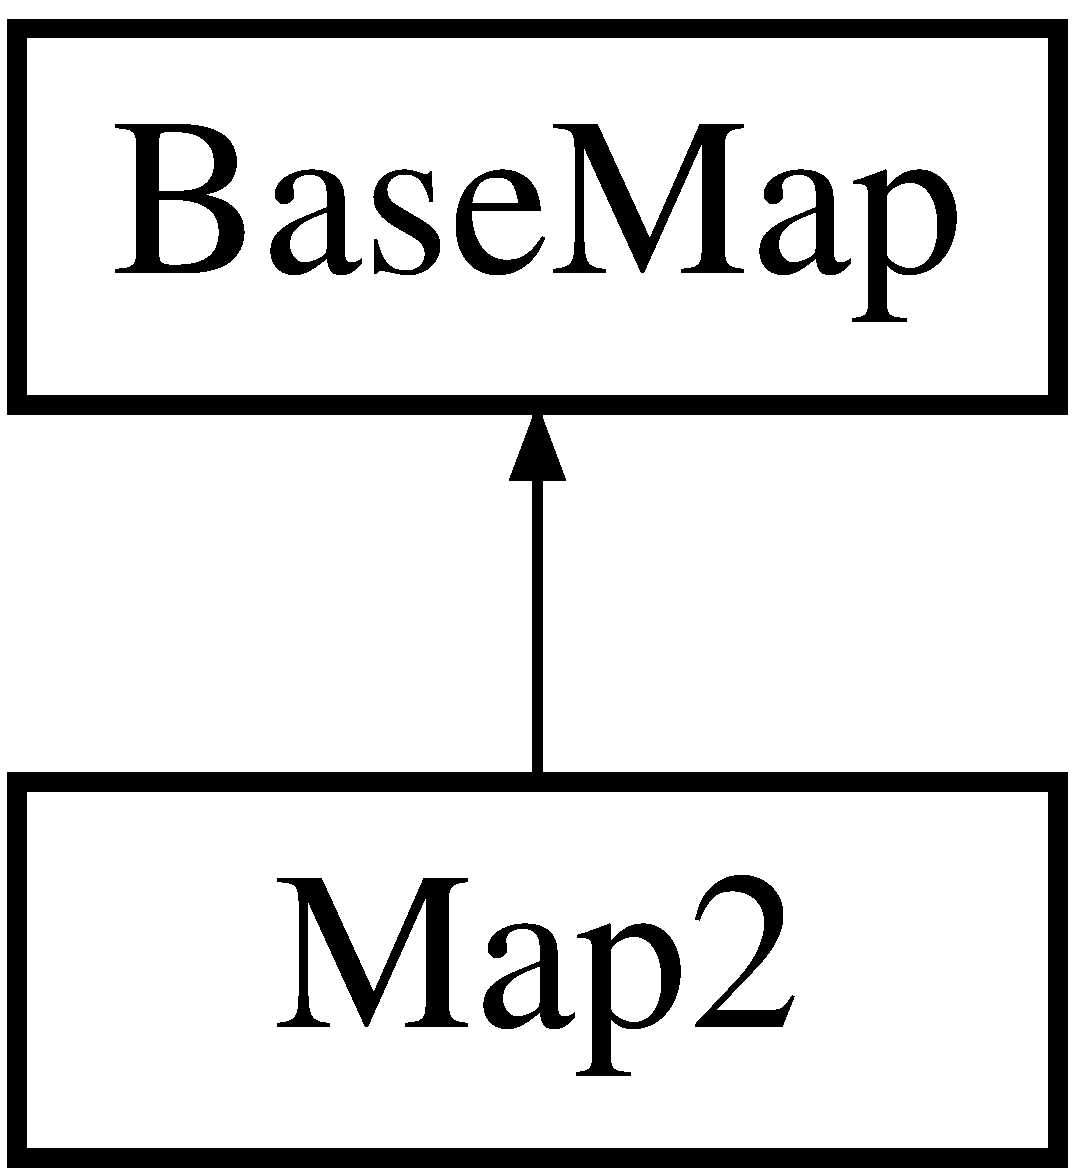
\includegraphics[height=2.000000cm]{class_map2}
\end{center}
\end{figure}
\subsection*{Public Member Functions}
\begin{DoxyCompactItemize}
\item 
\hyperlink{class_map2_a1cb7f3d680636c4d1c66649ff0f88143}{Map2} ()
\begin{DoxyCompactList}\small\item\em Constructor of \hyperlink{class_map2}{Map2} class. \end{DoxyCompactList}\end{DoxyCompactItemize}
\subsection*{Additional Inherited Members}


\subsection{Constructor \& Destructor Documentation}
\mbox{\Hypertarget{class_map2_a1cb7f3d680636c4d1c66649ff0f88143}\label{class_map2_a1cb7f3d680636c4d1c66649ff0f88143}} 
\index{Map2@{Map2}!Map2@{Map2}}
\index{Map2@{Map2}!Map2@{Map2}}
\subsubsection{\texorpdfstring{Map2()}{Map2()}}
{\footnotesize\ttfamily Map2\+::\+Map2 (\begin{DoxyParamCaption}{ }\end{DoxyParamCaption})}



Constructor of \hyperlink{class_map2}{Map2} class. 


\begin{DoxyParams}{Parameters}
{\em none} & \\
\hline
\end{DoxyParams}
\begin{DoxyReturn}{Returns}
none 
\end{DoxyReturn}


The documentation for this class was generated from the following files\+:\begin{DoxyCompactItemize}
\item 
D\+:/\+R\+C\+C/\+C\+I\+S17\+A/\+Mac\+Nhan\+\_\+44051/\+Proj/\+Project\+\_\+2/\+Project2/Map2.\+h\item 
D\+:/\+R\+C\+C/\+C\+I\+S17\+A/\+Mac\+Nhan\+\_\+44051/\+Proj/\+Project\+\_\+2/\+Project2/Map2.\+cpp\end{DoxyCompactItemize}

\hypertarget{class_map3}{}\section{Map3 Class Reference}
\label{class_map3}\index{Map3@{Map3}}
Inheritance diagram for Map3\+:\begin{figure}[H]
\begin{center}
\leavevmode
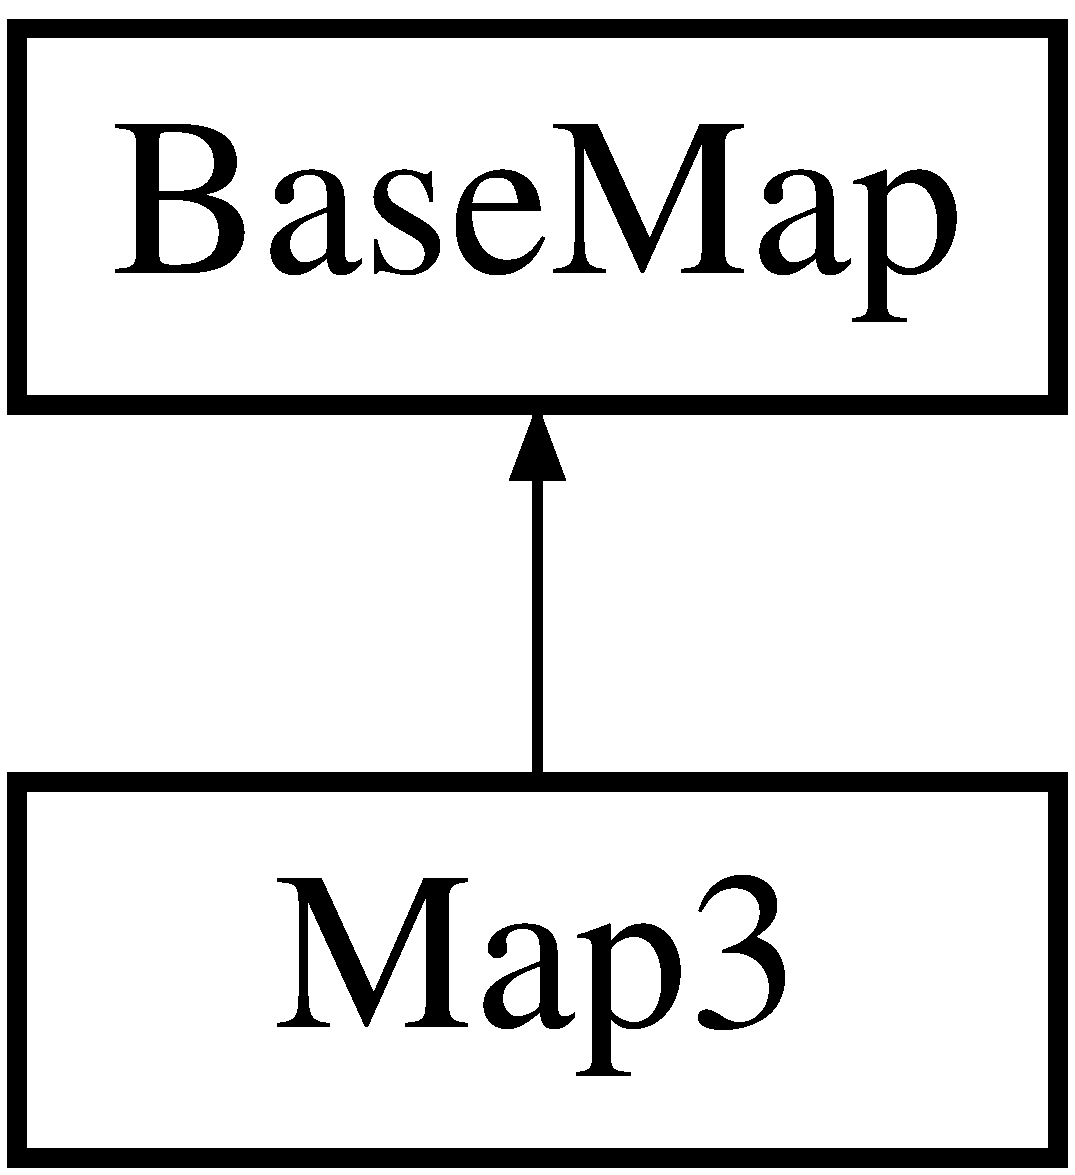
\includegraphics[height=2.000000cm]{class_map3}
\end{center}
\end{figure}
\subsection*{Public Member Functions}
\begin{DoxyCompactItemize}
\item 
\hyperlink{class_map3_a11d68f6bbc7324970f6f433d284711e3}{Map3} ()
\begin{DoxyCompactList}\small\item\em Constructor of \hyperlink{class_map3}{Map3} class. \end{DoxyCompactList}\end{DoxyCompactItemize}
\subsection*{Additional Inherited Members}


\subsection{Constructor \& Destructor Documentation}
\mbox{\Hypertarget{class_map3_a11d68f6bbc7324970f6f433d284711e3}\label{class_map3_a11d68f6bbc7324970f6f433d284711e3}} 
\index{Map3@{Map3}!Map3@{Map3}}
\index{Map3@{Map3}!Map3@{Map3}}
\subsubsection{\texorpdfstring{Map3()}{Map3()}}
{\footnotesize\ttfamily Map3\+::\+Map3 (\begin{DoxyParamCaption}{ }\end{DoxyParamCaption})}



Constructor of \hyperlink{class_map3}{Map3} class. 


\begin{DoxyParams}{Parameters}
{\em none} & \\
\hline
\end{DoxyParams}
\begin{DoxyReturn}{Returns}
none 
\end{DoxyReturn}


The documentation for this class was generated from the following files\+:\begin{DoxyCompactItemize}
\item 
D\+:/\+R\+C\+C/\+C\+I\+S17\+A/\+Mac\+Nhan\+\_\+44051/\+Proj/\+Project\+\_\+2/\+Project2/Map3.\+h\item 
D\+:/\+R\+C\+C/\+C\+I\+S17\+A/\+Mac\+Nhan\+\_\+44051/\+Proj/\+Project\+\_\+2/\+Project2/Map3.\+cpp\end{DoxyCompactItemize}

\hypertarget{class_object}{}\section{Object Class Reference}
\label{class_object}\index{Object@{Object}}
Inheritance diagram for Object\+:\begin{figure}[H]
\begin{center}
\leavevmode
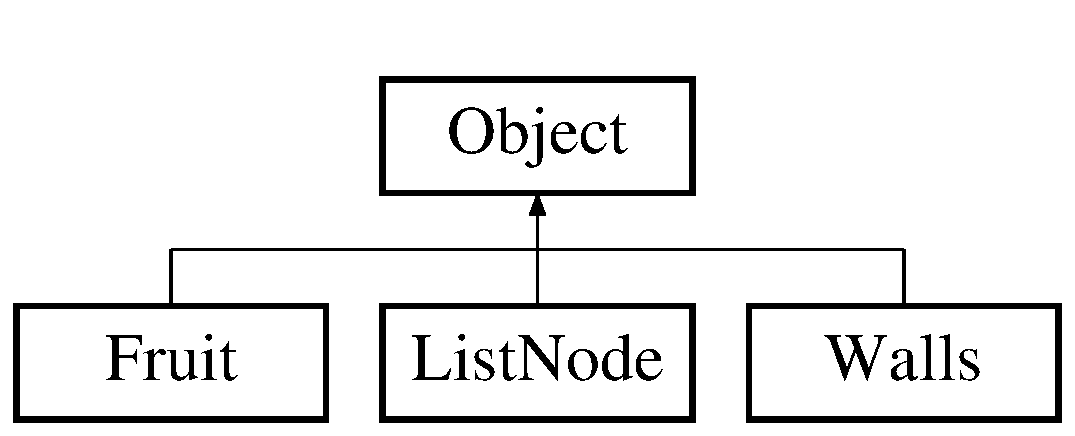
\includegraphics[height=2.000000cm]{class_object}
\end{center}
\end{figure}
\subsection*{Public Member Functions}
\begin{DoxyCompactItemize}
\item 
\hyperlink{class_object_a40860402e64d8008fb42329df7097cdb}{Object} ()
\begin{DoxyCompactList}\small\item\em Constructor of \hyperlink{class_object}{Object} class. \end{DoxyCompactList}\item 
void \hyperlink{class_object_a9b3c3653717b0540dfa783bf666abf63}{setY} (int)
\begin{DoxyCompactList}\small\item\em set the value of Coordinates Y \end{DoxyCompactList}\item 
int \hyperlink{class_object_a81accadc2226d0e6c41c09dccc7a5f5e}{getY} () const
\begin{DoxyCompactList}\small\item\em Get the Coordinates Y. \end{DoxyCompactList}\item 
void \hyperlink{class_object_ad62efaa642d05c8b54b4427c23803398}{setX} (int)
\begin{DoxyCompactList}\small\item\em set the value of Coordinates X \end{DoxyCompactList}\item 
int \hyperlink{class_object_a66bac5f818d4d7c05aa457e246e4ca7b}{getX} () const
\begin{DoxyCompactList}\small\item\em Get the Coordinates X. \end{DoxyCompactList}\item 
char \hyperlink{class_object_a78ae01107b8544f5c4590afb90f38258}{get\+Symbol} () const
\begin{DoxyCompactList}\small\item\em Get the symbol. \end{DoxyCompactList}\item 
\mbox{\Hypertarget{class_object_a3003c5556506521b805e013f90e0d740}\label{class_object_a3003c5556506521b805e013f90e0d740}} 
void {\bfseries operator=} (const \hyperlink{class_object}{Object} \&)
\item 
void \hyperlink{class_object_a6ad44e8d6238a0246882864be6c83e8e}{set\+Points} (int points)
\begin{DoxyCompactList}\small\item\em set the value of points \end{DoxyCompactList}\item 
int \hyperlink{class_object_a555148cd05b5b98d4d18b4cc5dc06a37}{get\+Points} () const
\begin{DoxyCompactList}\small\item\em Get the next node. \end{DoxyCompactList}\end{DoxyCompactItemize}
\subsection*{Protected Member Functions}
\begin{DoxyCompactItemize}
\item 
void \hyperlink{class_object_a7f524c95bbc774e71d692125d085be7e}{set\+Symbol} (char)
\begin{DoxyCompactList}\small\item\em set the value of symbol \end{DoxyCompactList}\end{DoxyCompactItemize}


\subsection{Constructor \& Destructor Documentation}
\mbox{\Hypertarget{class_object_a40860402e64d8008fb42329df7097cdb}\label{class_object_a40860402e64d8008fb42329df7097cdb}} 
\index{Object@{Object}!Object@{Object}}
\index{Object@{Object}!Object@{Object}}
\subsubsection{\texorpdfstring{Object()}{Object()}}
{\footnotesize\ttfamily Object\+::\+Object (\begin{DoxyParamCaption}{ }\end{DoxyParamCaption})}



Constructor of \hyperlink{class_object}{Object} class. 


\begin{DoxyParams}{Parameters}
{\em none} & \\
\hline
\end{DoxyParams}
\begin{DoxyReturn}{Returns}
none 
\end{DoxyReturn}


\subsection{Member Function Documentation}
\mbox{\Hypertarget{class_object_a555148cd05b5b98d4d18b4cc5dc06a37}\label{class_object_a555148cd05b5b98d4d18b4cc5dc06a37}} 
\index{Object@{Object}!get\+Points@{get\+Points}}
\index{get\+Points@{get\+Points}!Object@{Object}}
\subsubsection{\texorpdfstring{get\+Points()}{getPoints()}}
{\footnotesize\ttfamily int Object\+::get\+Points (\begin{DoxyParamCaption}{ }\end{DoxyParamCaption}) const}



Get the next node. 


\begin{DoxyParams}{Parameters}
{\em none} & \\
\hline
\end{DoxyParams}
\begin{DoxyReturn}{Returns}
none 
\end{DoxyReturn}
\mbox{\Hypertarget{class_object_a78ae01107b8544f5c4590afb90f38258}\label{class_object_a78ae01107b8544f5c4590afb90f38258}} 
\index{Object@{Object}!get\+Symbol@{get\+Symbol}}
\index{get\+Symbol@{get\+Symbol}!Object@{Object}}
\subsubsection{\texorpdfstring{get\+Symbol()}{getSymbol()}}
{\footnotesize\ttfamily char Object\+::get\+Symbol (\begin{DoxyParamCaption}{ }\end{DoxyParamCaption}) const}



Get the symbol. 


\begin{DoxyParams}{Parameters}
{\em none} & \\
\hline
\end{DoxyParams}
\begin{DoxyReturn}{Returns}
none 
\end{DoxyReturn}
\mbox{\Hypertarget{class_object_a66bac5f818d4d7c05aa457e246e4ca7b}\label{class_object_a66bac5f818d4d7c05aa457e246e4ca7b}} 
\index{Object@{Object}!getX@{getX}}
\index{getX@{getX}!Object@{Object}}
\subsubsection{\texorpdfstring{get\+X()}{getX()}}
{\footnotesize\ttfamily int Object\+::getX (\begin{DoxyParamCaption}{ }\end{DoxyParamCaption}) const}



Get the Coordinates X. 


\begin{DoxyParams}{Parameters}
{\em none} & \\
\hline
\end{DoxyParams}
\begin{DoxyReturn}{Returns}
none 
\end{DoxyReturn}
\mbox{\Hypertarget{class_object_a81accadc2226d0e6c41c09dccc7a5f5e}\label{class_object_a81accadc2226d0e6c41c09dccc7a5f5e}} 
\index{Object@{Object}!getY@{getY}}
\index{getY@{getY}!Object@{Object}}
\subsubsection{\texorpdfstring{get\+Y()}{getY()}}
{\footnotesize\ttfamily int Object\+::getY (\begin{DoxyParamCaption}{ }\end{DoxyParamCaption}) const}



Get the Coordinates Y. 


\begin{DoxyParams}{Parameters}
{\em none} & \\
\hline
\end{DoxyParams}
\begin{DoxyReturn}{Returns}
none 
\end{DoxyReturn}
\mbox{\Hypertarget{class_object_a6ad44e8d6238a0246882864be6c83e8e}\label{class_object_a6ad44e8d6238a0246882864be6c83e8e}} 
\index{Object@{Object}!set\+Points@{set\+Points}}
\index{set\+Points@{set\+Points}!Object@{Object}}
\subsubsection{\texorpdfstring{set\+Points()}{setPoints()}}
{\footnotesize\ttfamily void Object\+::set\+Points (\begin{DoxyParamCaption}\item[{int}]{points }\end{DoxyParamCaption})}



set the value of points 


\begin{DoxyParams}{Parameters}
{\em point} & -\/ The value of points \\
\hline
\end{DoxyParams}
\begin{DoxyReturn}{Returns}
none 
\end{DoxyReturn}
\mbox{\Hypertarget{class_object_a7f524c95bbc774e71d692125d085be7e}\label{class_object_a7f524c95bbc774e71d692125d085be7e}} 
\index{Object@{Object}!set\+Symbol@{set\+Symbol}}
\index{set\+Symbol@{set\+Symbol}!Object@{Object}}
\subsubsection{\texorpdfstring{set\+Symbol()}{setSymbol()}}
{\footnotesize\ttfamily void Object\+::set\+Symbol (\begin{DoxyParamCaption}\item[{char}]{symbol }\end{DoxyParamCaption})\hspace{0.3cm}{\ttfamily [protected]}}



set the value of symbol 


\begin{DoxyParams}{Parameters}
{\em symbol} & -\/ The value of symbol \\
\hline
\end{DoxyParams}
\begin{DoxyReturn}{Returns}
none 
\end{DoxyReturn}
\mbox{\Hypertarget{class_object_ad62efaa642d05c8b54b4427c23803398}\label{class_object_ad62efaa642d05c8b54b4427c23803398}} 
\index{Object@{Object}!setX@{setX}}
\index{setX@{setX}!Object@{Object}}
\subsubsection{\texorpdfstring{set\+X()}{setX()}}
{\footnotesize\ttfamily void Object\+::setX (\begin{DoxyParamCaption}\item[{int}]{x }\end{DoxyParamCaption})}



set the value of Coordinates X 


\begin{DoxyParams}{Parameters}
{\em X} & -\/ The value of Coordinates X \\
\hline
\end{DoxyParams}
\begin{DoxyReturn}{Returns}
none 
\end{DoxyReturn}
\mbox{\Hypertarget{class_object_a9b3c3653717b0540dfa783bf666abf63}\label{class_object_a9b3c3653717b0540dfa783bf666abf63}} 
\index{Object@{Object}!setY@{setY}}
\index{setY@{setY}!Object@{Object}}
\subsubsection{\texorpdfstring{set\+Y()}{setY()}}
{\footnotesize\ttfamily void Object\+::setY (\begin{DoxyParamCaption}\item[{int}]{y }\end{DoxyParamCaption})}



set the value of Coordinates Y 


\begin{DoxyParams}{Parameters}
{\em Y} & -\/ The value of Coordinates Y \\
\hline
\end{DoxyParams}
\begin{DoxyReturn}{Returns}
none 
\end{DoxyReturn}


The documentation for this class was generated from the following files\+:\begin{DoxyCompactItemize}
\item 
D\+:/\+R\+C\+C/\+C\+I\+S17\+A/\+Mac\+Nhan\+\_\+44051/\+Proj/\+Project\+\_\+2/\+Project2/Object.\+h\item 
D\+:/\+R\+C\+C/\+C\+I\+S17\+A/\+Mac\+Nhan\+\_\+44051/\+Proj/\+Project\+\_\+2/\+Project2/Object.\+cpp\end{DoxyCompactItemize}

\hypertarget{struct_scores}{}\section{Scores Struct Reference}
\label{struct_scores}\index{Scores@{Scores}}
\subsection*{Public Attributes}
\begin{DoxyCompactItemize}
\item 
int \hyperlink{struct_scores_aab2bf0fee1a8c2b6e85862c526ddbfae}{rank}
\item 
char \hyperlink{struct_scores_adc73cbe7efd07c64771ce7b0ef6c8a74}{name} \mbox{[}100\mbox{]}
\item 
int \hyperlink{struct_scores_adc160fc30f754360378856a273fef5e2}{scores}
\end{DoxyCompactItemize}


\subsection{Member Data Documentation}
\mbox{\Hypertarget{struct_scores_adc73cbe7efd07c64771ce7b0ef6c8a74}\label{struct_scores_adc73cbe7efd07c64771ce7b0ef6c8a74}} 
\index{Scores@{Scores}!name@{name}}
\index{name@{name}!Scores@{Scores}}
\subsubsection{\texorpdfstring{name}{name}}
{\footnotesize\ttfamily char Scores\+::name\mbox{[}100\mbox{]}}

Name of user \mbox{\Hypertarget{struct_scores_aab2bf0fee1a8c2b6e85862c526ddbfae}\label{struct_scores_aab2bf0fee1a8c2b6e85862c526ddbfae}} 
\index{Scores@{Scores}!rank@{rank}}
\index{rank@{rank}!Scores@{Scores}}
\subsubsection{\texorpdfstring{rank}{rank}}
{\footnotesize\ttfamily int Scores\+::rank}

The rank of user depend on score \mbox{\Hypertarget{struct_scores_adc160fc30f754360378856a273fef5e2}\label{struct_scores_adc160fc30f754360378856a273fef5e2}} 
\index{Scores@{Scores}!scores@{scores}}
\index{scores@{scores}!Scores@{Scores}}
\subsubsection{\texorpdfstring{scores}{scores}}
{\footnotesize\ttfamily int Scores\+::scores}

Score of user 

The documentation for this struct was generated from the following file\+:\begin{DoxyCompactItemize}
\item 
\hyperlink{_scores_8h}{Scores.\+h}\end{DoxyCompactItemize}

\hypertarget{class_snake}{}\section{Snake Class Reference}
\label{class_snake}\index{Snake@{Snake}}
\subsection*{Public Types}
\begin{DoxyCompactItemize}
\item 
\mbox{\Hypertarget{class_snake_af0cc1dc5acd878a6530198ba11d701f4}\label{class_snake_af0cc1dc5acd878a6530198ba11d701f4}} 
enum {\bfseries move\+State} \{ {\bfseries UP}, 
{\bfseries D\+O\+WN}, 
{\bfseries L\+E\+FT}, 
{\bfseries R\+I\+G\+HT}
 \}
\end{DoxyCompactItemize}
\subsection*{Public Member Functions}
\begin{DoxyCompactItemize}
\item 
\hyperlink{class_snake_aa9cbcdb4b25d84cbf83509039cac8d01}{Snake} ()
\begin{DoxyCompactList}\small\item\em Constructor of \hyperlink{class_snake}{Snake} class. \end{DoxyCompactList}\item 
void \hyperlink{class_snake_ac9f00db4b693de3c552a0ae7275c8412}{init} ()
\begin{DoxyCompactList}\small\item\em Create value for snake. \end{DoxyCompactList}\item 
void \hyperlink{class_snake_a5aea260c328ba4f8701539eab08283d9}{move} ()
\begin{DoxyCompactList}\small\item\em Move snake to other position. \end{DoxyCompactList}\item 
int \hyperlink{class_snake_a9dd0a8a2a763668e12646385da8280e2}{size} ()
\begin{DoxyCompactList}\small\item\em The size of snake. \end{DoxyCompactList}\item 
void \hyperlink{class_snake_a2940bb3101863ab8a02a8a396c6552f2}{insert\+Back} ()
\begin{DoxyCompactList}\small\item\em Insert node to back of list. \end{DoxyCompactList}\item 
void \hyperlink{class_snake_aef36368de7f3f811d424e3ae02f2393d}{delete\+Back} ()
\begin{DoxyCompactList}\small\item\em Delete node at back of list. \end{DoxyCompactList}\item 
\mbox{\Hypertarget{class_snake_a06a611ba3edd353051e4dcd59642ace0}\label{class_snake_a06a611ba3edd353051e4dcd59642ace0}} 
void {\bfseries display\+List} () const
\item 
\hyperlink{class_list_node}{List\+Node} $\ast$ \hyperlink{class_snake_a69f6fbdc2ef89a8d8881dbfdbca2260f}{get\+Head} () const
\begin{DoxyCompactList}\small\item\em Get list head pointer. \end{DoxyCompactList}\item 
void \hyperlink{class_snake_a1d32911132c48ffb2cbe6752b5100405}{set\+Max\+Speed} (int max\+Speed)
\begin{DoxyCompactList}\small\item\em Set value of max speed. \end{DoxyCompactList}\item 
int \hyperlink{class_snake_ae70820c279a79caae3dcfe4cbaa4b747}{get\+Max\+Speed} () const
\begin{DoxyCompactList}\small\item\em Get max speed. \end{DoxyCompactList}\end{DoxyCompactItemize}
\subsection*{Public Attributes}
\begin{DoxyCompactItemize}
\item 
move\+State \hyperlink{class_snake_a55f2ac9d5eb97c9f86b001d47ce0e8dc}{state}
\end{DoxyCompactItemize}


\subsection{Constructor \& Destructor Documentation}
\mbox{\Hypertarget{class_snake_aa9cbcdb4b25d84cbf83509039cac8d01}\label{class_snake_aa9cbcdb4b25d84cbf83509039cac8d01}} 
\index{Snake@{Snake}!Snake@{Snake}}
\index{Snake@{Snake}!Snake@{Snake}}
\subsubsection{\texorpdfstring{Snake()}{Snake()}}
{\footnotesize\ttfamily Snake\+::\+Snake (\begin{DoxyParamCaption}{ }\end{DoxyParamCaption})}



Constructor of \hyperlink{class_snake}{Snake} class. 


\begin{DoxyParams}{Parameters}
{\em none} & \\
\hline
\end{DoxyParams}
\begin{DoxyReturn}{Returns}
none 
\end{DoxyReturn}


\subsection{Member Function Documentation}
\mbox{\Hypertarget{class_snake_aef36368de7f3f811d424e3ae02f2393d}\label{class_snake_aef36368de7f3f811d424e3ae02f2393d}} 
\index{Snake@{Snake}!delete\+Back@{delete\+Back}}
\index{delete\+Back@{delete\+Back}!Snake@{Snake}}
\subsubsection{\texorpdfstring{delete\+Back()}{deleteBack()}}
{\footnotesize\ttfamily void Snake\+::delete\+Back (\begin{DoxyParamCaption}{ }\end{DoxyParamCaption})}



Delete node at back of list. 


\begin{DoxyParams}{Parameters}
{\em none} & \\
\hline
\end{DoxyParams}
\begin{DoxyReturn}{Returns}
none 
\end{DoxyReturn}
\mbox{\Hypertarget{class_snake_a69f6fbdc2ef89a8d8881dbfdbca2260f}\label{class_snake_a69f6fbdc2ef89a8d8881dbfdbca2260f}} 
\index{Snake@{Snake}!get\+Head@{get\+Head}}
\index{get\+Head@{get\+Head}!Snake@{Snake}}
\subsubsection{\texorpdfstring{get\+Head()}{getHead()}}
{\footnotesize\ttfamily \hyperlink{class_list_node}{List\+Node} $\ast$ Snake\+::get\+Head (\begin{DoxyParamCaption}{ }\end{DoxyParamCaption}) const}



Get list head pointer. 


\begin{DoxyParams}{Parameters}
{\em none} & \\
\hline
\end{DoxyParams}
\begin{DoxyReturn}{Returns}
List head pointer 
\end{DoxyReturn}
\mbox{\Hypertarget{class_snake_ae70820c279a79caae3dcfe4cbaa4b747}\label{class_snake_ae70820c279a79caae3dcfe4cbaa4b747}} 
\index{Snake@{Snake}!get\+Max\+Speed@{get\+Max\+Speed}}
\index{get\+Max\+Speed@{get\+Max\+Speed}!Snake@{Snake}}
\subsubsection{\texorpdfstring{get\+Max\+Speed()}{getMaxSpeed()}}
{\footnotesize\ttfamily int Snake\+::get\+Max\+Speed (\begin{DoxyParamCaption}{ }\end{DoxyParamCaption}) const}



Get max speed. 


\begin{DoxyParams}{Parameters}
{\em none} & \\
\hline
\end{DoxyParams}
\begin{DoxyReturn}{Returns}
max\+Speed 
\end{DoxyReturn}
\mbox{\Hypertarget{class_snake_ac9f00db4b693de3c552a0ae7275c8412}\label{class_snake_ac9f00db4b693de3c552a0ae7275c8412}} 
\index{Snake@{Snake}!init@{init}}
\index{init@{init}!Snake@{Snake}}
\subsubsection{\texorpdfstring{init()}{init()}}
{\footnotesize\ttfamily void Snake\+::init (\begin{DoxyParamCaption}{ }\end{DoxyParamCaption})}



Create value for snake. 


\begin{DoxyParams}{Parameters}
{\em none} & \\
\hline
\end{DoxyParams}
\begin{DoxyReturn}{Returns}
none 
\end{DoxyReturn}
\mbox{\Hypertarget{class_snake_a2940bb3101863ab8a02a8a396c6552f2}\label{class_snake_a2940bb3101863ab8a02a8a396c6552f2}} 
\index{Snake@{Snake}!insert\+Back@{insert\+Back}}
\index{insert\+Back@{insert\+Back}!Snake@{Snake}}
\subsubsection{\texorpdfstring{insert\+Back()}{insertBack()}}
{\footnotesize\ttfamily void Snake\+::insert\+Back (\begin{DoxyParamCaption}{ }\end{DoxyParamCaption})}



Insert node to back of list. 


\begin{DoxyParams}{Parameters}
{\em none} & \\
\hline
\end{DoxyParams}
\begin{DoxyReturn}{Returns}
none 
\end{DoxyReturn}
\mbox{\Hypertarget{class_snake_a5aea260c328ba4f8701539eab08283d9}\label{class_snake_a5aea260c328ba4f8701539eab08283d9}} 
\index{Snake@{Snake}!move@{move}}
\index{move@{move}!Snake@{Snake}}
\subsubsection{\texorpdfstring{move()}{move()}}
{\footnotesize\ttfamily void Snake\+::move (\begin{DoxyParamCaption}{ }\end{DoxyParamCaption})}



Move snake to other position. 


\begin{DoxyParams}{Parameters}
{\em none} & \\
\hline
\end{DoxyParams}
\begin{DoxyReturn}{Returns}
none 
\end{DoxyReturn}
\mbox{\Hypertarget{class_snake_a1d32911132c48ffb2cbe6752b5100405}\label{class_snake_a1d32911132c48ffb2cbe6752b5100405}} 
\index{Snake@{Snake}!set\+Max\+Speed@{set\+Max\+Speed}}
\index{set\+Max\+Speed@{set\+Max\+Speed}!Snake@{Snake}}
\subsubsection{\texorpdfstring{set\+Max\+Speed()}{setMaxSpeed()}}
{\footnotesize\ttfamily void Snake\+::set\+Max\+Speed (\begin{DoxyParamCaption}\item[{int}]{max\+Speed }\end{DoxyParamCaption})}



Set value of max speed. 


\begin{DoxyParams}{Parameters}
{\em max\+Speed} & -\/ value of max speed \\
\hline
\end{DoxyParams}
\begin{DoxyReturn}{Returns}
none 
\end{DoxyReturn}
\mbox{\Hypertarget{class_snake_a9dd0a8a2a763668e12646385da8280e2}\label{class_snake_a9dd0a8a2a763668e12646385da8280e2}} 
\index{Snake@{Snake}!size@{size}}
\index{size@{size}!Snake@{Snake}}
\subsubsection{\texorpdfstring{size()}{size()}}
{\footnotesize\ttfamily int Snake\+::size (\begin{DoxyParamCaption}{ }\end{DoxyParamCaption})}



The size of snake. 


\begin{DoxyParams}{Parameters}
{\em none} & \\
\hline
\end{DoxyParams}
\begin{DoxyReturn}{Returns}
the size of snake 
\end{DoxyReturn}


\subsection{Member Data Documentation}
\mbox{\Hypertarget{class_snake_a55f2ac9d5eb97c9f86b001d47ce0e8dc}\label{class_snake_a55f2ac9d5eb97c9f86b001d47ce0e8dc}} 
\index{Snake@{Snake}!state@{state}}
\index{state@{state}!Snake@{Snake}}
\subsubsection{\texorpdfstring{state}{state}}
{\footnotesize\ttfamily move\+State Snake\+::state}

Direction of snake 

The documentation for this class was generated from the following files\+:\begin{DoxyCompactItemize}
\item 
D\+:/\+R\+C\+C/\+C\+I\+S17\+A/\+Mac\+Nhan\+\_\+44051/\+Proj/\+Project\+\_\+2/\+Project2/Snake.\+h\item 
D\+:/\+R\+C\+C/\+C\+I\+S17\+A/\+Mac\+Nhan\+\_\+44051/\+Proj/\+Project\+\_\+2/\+Project2/Snake.\+cpp\end{DoxyCompactItemize}

\hypertarget{class_walls}{}\section{Walls Class Reference}
\label{class_walls}\index{Walls@{Walls}}
Inheritance diagram for Walls\+:\begin{figure}[H]
\begin{center}
\leavevmode
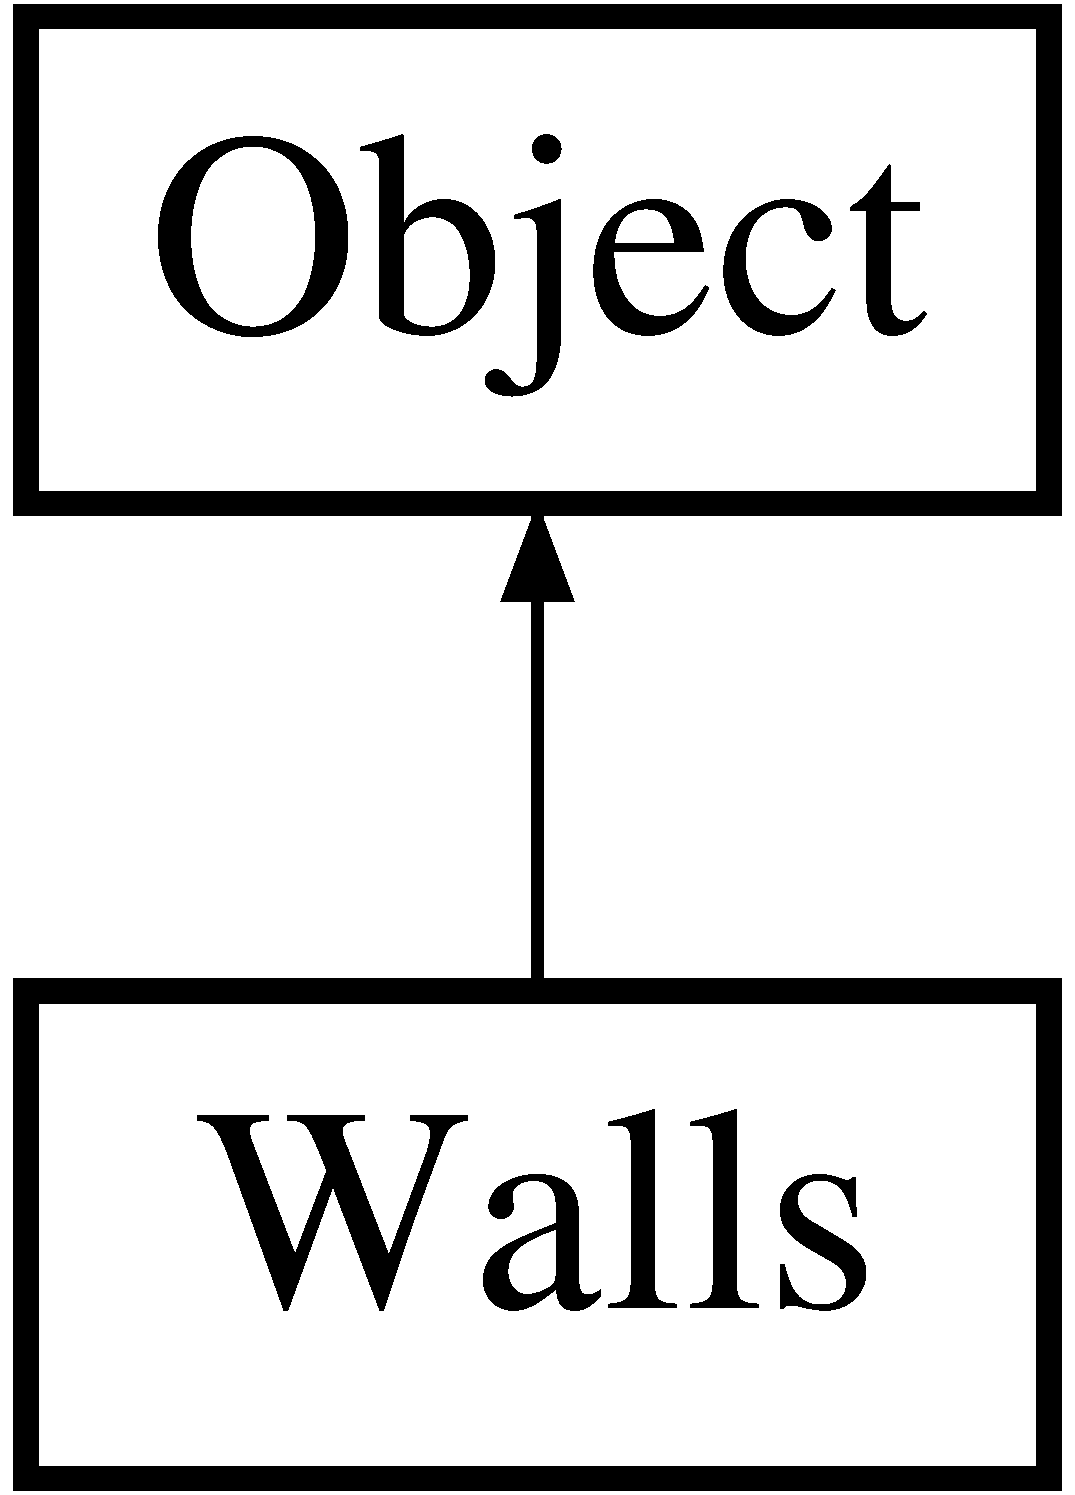
\includegraphics[height=2.000000cm]{class_walls}
\end{center}
\end{figure}
\subsection*{Public Member Functions}
\begin{DoxyCompactItemize}
\item 
\hyperlink{class_walls_aa6927c56b93d24169a8909e73ba5c72f}{Walls} ()
\begin{DoxyCompactList}\small\item\em Constructor of \hyperlink{class_walls}{Walls} class. \end{DoxyCompactList}\end{DoxyCompactItemize}
\subsection*{Additional Inherited Members}


\subsection{Constructor \& Destructor Documentation}
\mbox{\Hypertarget{class_walls_aa6927c56b93d24169a8909e73ba5c72f}\label{class_walls_aa6927c56b93d24169a8909e73ba5c72f}} 
\index{Walls@{Walls}!Walls@{Walls}}
\index{Walls@{Walls}!Walls@{Walls}}
\subsubsection{\texorpdfstring{Walls()}{Walls()}}
{\footnotesize\ttfamily Walls\+::\+Walls (\begin{DoxyParamCaption}{ }\end{DoxyParamCaption})}



Constructor of \hyperlink{class_walls}{Walls} class. 


\begin{DoxyParams}{Parameters}
{\em none} & \\
\hline
\end{DoxyParams}
\begin{DoxyReturn}{Returns}
none 
\end{DoxyReturn}


The documentation for this class was generated from the following files\+:\begin{DoxyCompactItemize}
\item 
D\+:/\+R\+C\+C/\+C\+I\+S17\+A/\+Mac\+Nhan\+\_\+44051/\+Proj/\+Project\+\_\+2/\+Project2/Walls.\+h\item 
D\+:/\+R\+C\+C/\+C\+I\+S17\+A/\+Mac\+Nhan\+\_\+44051/\+Proj/\+Project\+\_\+2/\+Project2/Walls.\+cpp\end{DoxyCompactItemize}

%--- End generated contents ---

% Index
\backmatter
\newpage
\phantomsection
\clearemptydoublepage
\addcontentsline{toc}{chapter}{Index}
\printindex

\end{document}
